\documentclass[12pt]{article}
\usepackage[margin=1in]{geometry} 
\usepackage{amsmath,amsthm,amssymb,amsfonts,enumerate,listings,graphicx,epstopdf,siunitx}
\graphicspath{~/Documents/school/fall16/stat586/hw2}
 
\newcommand{\N}{\mathbb{N}}
\newcommand{\Z}{\mathbb{Z}}
 
\newenvironment{problem}[2][Problem]{\begin{trivlist}
\item[\hskip \labelsep {\bfseries #1}\hskip \labelsep {\bfseries #2.}]
  \vspace{1 cm}
}{\end{trivlist}}

\begin{document}
\title{Homework Set 2}
\author{Taylor Bodin}
\maketitle

\begin{problem}{3.1}
\item
  \begin{enumerate}[a.]
    \item %A
      Not a valid CDF because $F_X(x)$ decreases.
    \item %B
      This is a valid CDF since it satisfies all the properties of a CDF
    \item %C
      This is a valid CDF since it satisfies all the properties of a CDF
    \item %D
      Not a valid CDF because: $F_x(\infty) \neq 1$
  \end{enumerate}
\end{problem}

\begin{problem}{3.3}
\item
  $F_X(x) = \left(\frac{1}{2} + \frac{1}{\pi}\tan^{-1}(x)\right)u(x)$
  \begin{enumerate}[a.]
    \item %A
      $P(X < 2) = F_X(2) = .8524$
    \item %B
      $P(X>4) = 1-F_X(4) = 1 - (.9220) = \num{7.798e-2}$
    \item %C
      $P(1<x<3) = F_X(3) - F_X(1) = .8976 - .7500 = .1476$
    \item %D
      $P(X>2 | X<4) = \frac{P(X>2 \cap X<4)}{P(X<4)} = \frac{F_X(4)
      -F_X(2)}{F_X(4)} = \num{7.549e-2}$
  \end{enumerate} 
\end{problem}

\begin{problem}{3.5} %TODO: FIGURE A.
\item
  \begin{enumerate}[a.] 
    \item %A. TODO: FIGURE
%     \begin{figure}[htpb]
%       \centering
%       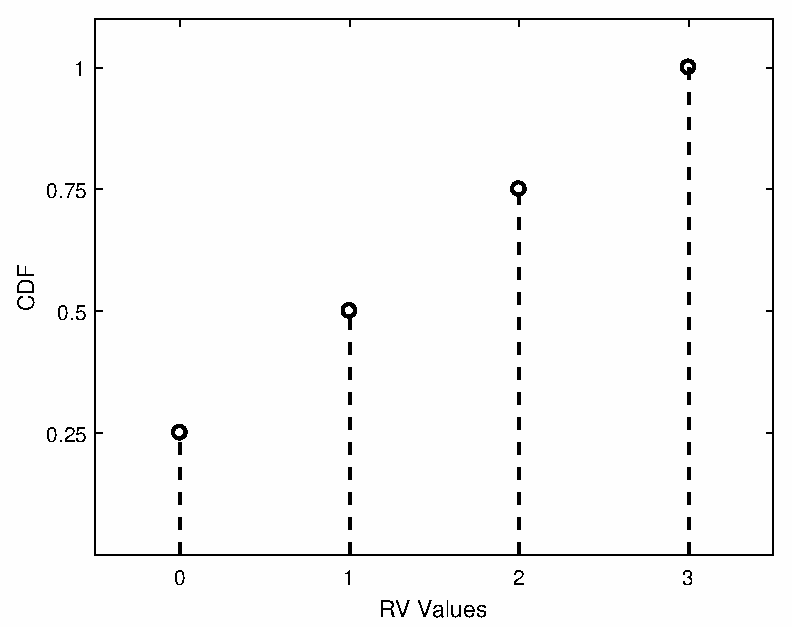
\includegraphics[width=\textwidth,height=\textheight,keepaspectratio]{fig_3_5.eps}
%       \caption{Problem 3.5, Sketch of the CDF of X}
%     \end{figure}
    \item %B.
      $F_X(x) = .25u(x) + .25u(x-1) + .25u(x-2) +.25u(x-3)$
  \end{enumerate}
\end{problem}

\begin{problem}{3.7}
\item
  \begin{enumerate}[a.]
    \item %A.
      Since $a_k$ is basically a PMF, it must satisfy the same conditions. \\
      Specifically, $\sum_{k=0}^\infty a_k = 1$ and $a_k \geq 0 \forall k$.
    \item %B.
      $P(X \leq n) = \sum_{k=0}^n a_k u(x-k)$
  \end{enumerate}
\end{problem}

\begin{problem}{3.9}
\item
  \begin{enumerate}[a.]
    \item %A.
      $P(X = 0) = F_X(0)-F_X(0) = 0, \\ P(X=1) = F_X(1)-F_X(1) = 0$
    \item %B
      $P(X < 0) = F_X(0) = \frac{1}{2}, \\
      P(X>\frac{1}{2}) = 1 - F_X(\frac{1}{2}) = 1-\frac{3}{4} = \frac{1}{4}$
    \item %C.
      $P(X>\frac{1}{2} | X > 0) = \frac{P((X > 0)\cap(X >\frac{1}{2}))}{P(X>0)}
      = \frac{P(X>\frac{1}{2})}{P(X>0)} = \frac{1-F_X(\frac{1}{2})}{1-F_X(0)} 
      = \frac{\frac{1}{4}}{\frac{1}{2}} = \frac{1}{2}$ 
  \end{enumerate}
\end{problem}

\begin{problem}{3.11} %TODO: FIGURES
\item
  \begin{enumerate}[a.]
    \item %A.
      \begin{align*}
        F_X(x) &= \int_{-\infty}^{x} 0dy(1-u(t)) + \int_{0}^{x} dy  \ u(t) \\
        &= 0 + y\big|_{y=0}^x \\
        &=\begin{cases}
            0 & x \leq 0 \\
            x & 0 < x \geq 1 \\
            1 & x > 1
          \end{cases}
      \end{align*}
    \item %TODO A. Figure
%     \begin{figure}[htpb]
%       \centering
%       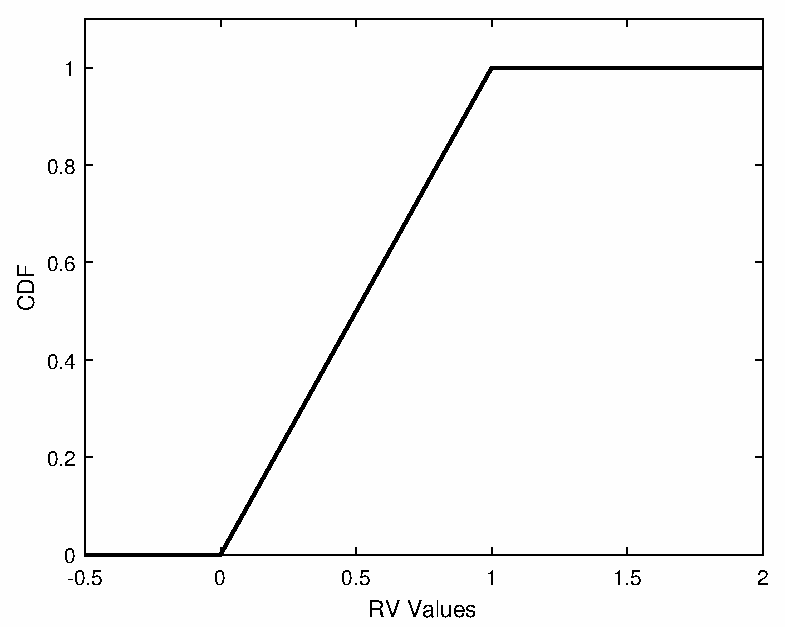
\includegraphics[width=\textwidth,height=\textheight,keepaspectratio]{fig_3_11_a.eps}
%       \caption{Problem 3.11 A, Sketch of the CDF of X}
%     \end{figure}
    \item %TODO B.
      \begin{align*}
        F_X(x) &= \int_{-\infty}^{x} 0 \ dy = 0 \\
          &+ \int_{0}^{x} y  dy \ (u(t)-u(t-1))) \\
          &+ \int_0^1 y  dy + \int_1^x (2-y)dy \ (u(t-2) - u(t-2)) \\
        &=\begin{cases}
            0 & x \leq 0 \\
            \frac{x^2}{2} & 0 < x \geq 1 \\
            -\frac{x^2}{2} + 2x - 1 & 1 > x \geq 2 \\
            1 & x > 2
          \end{cases}
      \end{align*}
    \item %TODO B. Figure
%     \begin{figure}[htpb]
%       \centering
%       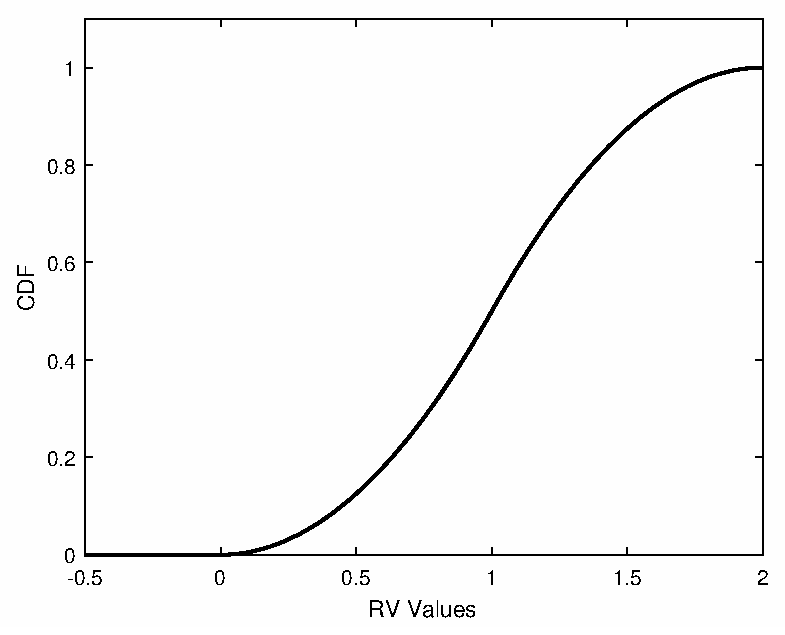
\includegraphics[width=\textwidth,height=\textheight,keepaspectratio]{fig_3_11_b.eps}
%       \caption{Problem 3.11 B, Sketch of the CDF of X}
%     \end{figure}
  \end{enumerate}
\end{problem}

\begin{problem}{3.13}
\item
  \begin{enumerate}[a.]
    \item %A. 
      $f_X(x)$ is of the form of a exponential random variable. Therefore,
      c is known to be equal to the coefficient of the exponent multiplied
      by negative 1. Thus, $c = 2$. The CDF is also known to be 
      $F_X(x) = \left[1 - e^{-\frac{x}{b}}\right]u(x)$ and is used for the 
      following problems. 
    \item %B.
      $P(X>2) = 1 - F_X(2) = 1 - .8647 = .1353$
    \item %C.
      $P(X<3) = F_X(3) = .9975$
    \item %D.
      $P(X < 3|X>2) = \frac{P(X<3)\cap P(X>2)}{P(X>2)}
      = \frac{F_X(3) - F_X(2)}{F_X(2)} = \num{1.613e-2}$
  \end{enumerate}
\end{problem}

\begin{problem}{3.15}
\item
  \begin{enumerate}[a.]
    \item %A.
      The CDF: $F_X(X) = \frac{2\sin^{-1}(\frac{x}{5})+\pi}{2\pi}$
      \begin{align*}
        1 &= \int_{-5}^5 \frac{c}{\sqrt{25-x^2}}dx \\
        &= c\sin^{-1}\left( \frac{x}{5} \right) + c\frac{\pi}{2}\big|_{-5}^5 \\
        &= c\left[ \sin^{-1}(1) + \frac{\pi}{2} - \sin^{-1} - \frac{pi}{2} \right] \\
        &= c\left[ \frac{\pi}{2} - (-\frac{\pi}{2})\right] \\
        c &= \frac{1}{\pi}
      \end{align*}
    \item %B.
      $P(X>2) = 1 - F_X(2) = 1 - .6310 = .3690$
    \item %C.
      $P(X<3) = F_X(3) = .7048$
    \item %D.
      $P(X < 3|X>2) = \frac{P(X<3)\cap P(X>2)}{P(X>2)}
      = \frac{F_X(3) - F_X(2)}{F_X(2)} = .1170$
  \end{enumerate}
\end{problem}

\begin{problem}{3.17}
\item
  \begin{enumerate}[a.]
    \item %A.
      $f_x \geq 0 \ \forall \ x$ and $\int_{-\infty}^{\infty} f_x(x)dx = 1$.
      Therefore, $f_x$ is a valid PDF.
    \item %B.
      $f_x \geq 0 \ \forall \ x$ but $\int_{-\infty}^{\infty} f_x(x)dx \approx 1.333$.
      Therefore, $f_x$ is not a valid PDF.
    \item %C.
      $f_x \geq 0 \ \forall \ x$ but $\int_{-\infty}^{\infty} f_x(x)dx =
      \frac{1}{4}$. Therefore, $f_x$ is not a valid PDF.
    \item %D.
      $f_x \ngeq 0 \ \forall \ x$ and $\int_{-\infty}^{\infty} f_x(x)dx = 0$.
      Therefore, $f_x$ is not a valid PDF.
  \end{enumerate}
\end{problem}

\begin{problem}{3.19}
\item %A.
  \begin{align*}
    I &= \int_{-\infty}^{\infty} e^{-\frac{x^2}{2}}dx = \sqrt{2\pi} \\
    I^2 &= \left(\int_{-\infty}^{\infty} e^{-\frac{x^2}{2}}dx \right)
    \left( \int_{-\infty}^{\infty} e^{-\frac{y^2}{2}}dy \right) = 2\pi \\
    &= \int_{-\infty}^{\infty} \int_{-\infty}^{\infty} e^{-\frac{x^2+y^2}{2}}dydx
    & & \textrm{Transform to polar coordinates} \\
    &= \int_{0}^{2\pi} \int_{0}^{\rho} e^{-\frac{\rho^2}{2}}\rho d\rho d\theta \\
    &= \int_{0}^{2\pi} \int_{a}^{b} -e^{u}du d\theta & & u = -\frac{\rho^2}{2} \\
    &= \int_{0}^{2\pi} -e^{-\frac{\rho}{2}} \big|_{\rho = 0}^{\infty} d\theta \\
    &= \int_{0}^{2\pi} d\theta \\
    &= 2\pi
  \end{align*}
\end{problem}

\begin{problem}{3.21}
\item
  \begin{enumerate}[a.]
    \item %A.
      \begin{align*}
        1 &= c \int_{-\infty}^{\infty} e^{-2x^2 -3x-1)}dx \\
        &= c \int_{-\infty}^{\infty} e^{-2(x^2 -\frac{3}{2}x-\frac{1}{2})}dx \\
        &= c \int_{-\infty}^{\infty} e^{-2(x +\frac{3}{4})^2-\frac{3}{4}^2+\frac{1}{2})}dx \\
        &= ce^{-2\left(-(\frac{3}{4})^2+\frac{1}{2}\right)} \int_{-\infty}^{\infty} e^{-2(x +\frac{3}{4})^2}dx \\
        &= ce^{\frac{1}{8}} \int_{-\infty}^{\infty} e^{-2(x +\frac{3}{4})^2}dx \\
      \end{align*}
    \item %B.
      Now that the Gaussian is in a more familiar form, $m$ and $\sigma$ can be
      determined by inspection. \\
      $m = -\frac{3}{4}, \sigma = \frac{1}{\sqrt{4}}$
    \item %C.
      Using $m$ and $\sigma$, one can set $ce^{\frac{1}{8}}= \frac{1}{\sqrt{2\pi\sigma^2}}$.
      Solving for c,\\
      $\frac{\sqrt{\frac{2}{\pi}}}{\sqrt[8]{e}} \approx .7041$
  \end{enumerate}
\end{problem}

\begin{problem}{3.23}
\item
  \begin{enumerate}[a.]
    \item %a.
      $P(x>0) = Q\left(\frac{0-(-1)}{\sqrt{\frac{1}{4}}}\right) \\ = Q(2)$
    \item %b.
      $P(x>2) = Q\left(\frac{2-(-1)}{\sqrt{\frac{1}{4}}}\right) \\ = Q(6)$
    \item %c.
      $P(x<-3) = 1 -Q\left(\frac{-3-(-1)}{\sqrt{\frac{1}{4}}}\right) \\ = 1-Q(-4) Q(4)$
    \item %d.
      $P(x<-4) = 1 -Q\left(\frac{-4-(-1)}{\sqrt{\frac{1}{4}}}\right) = 1-Q(-6) \\ = Q(6)$
    \item %e.
      $P(|x+1|>3) = P(x<-4 \cup x>2) = P(x>2) + P(x<-4) \\ = Q(2)+Q(6)$
    \item %f.
      $P(|x+1|<2) = P(-3<x<1) = P(x>-3) - P(x>1) = Q\left(\frac{-3-(-1)}{\sqrt{\frac{1}{4}}}\right)
      - Q\left(\frac{1-(-1)}{\sqrt{\frac{1}{4}}}\right) = Q(-4)-Q(4) = 1-2Q(4)$
    \item %g.
      $P(|x+2|>1) = P(x<-4 \cup x>0) = P(x<-4) + P(x>0) = Q\left(\frac{0-(-1)}{\sqrt{\frac{1}{4}}}\right)
      + 1 - Q\left(\frac{-4-(-1)}{\sqrt{\frac{1}{4}}}\right) = Q(2) + (1 - Q(-6)) = Q(2)+Q(6)$
    \item %h.
      $P(|x-1|<1) = P(-1<x<3) = P(x>-1) - P(x>3) = Q\left(\frac{-1-(-1)}{\sqrt{\frac{1}{4}}}\right)
      - Q\left(\frac{3-(-1)}{\sqrt{\frac{1}{4}}}\right) \\ = Q(2)-Q(8)$
  \end{enumerate}
\end{problem}

\begin{problem}{3.25}
\item
  \begin{align*}
    P(v \geq \SI{10}{\micro\volt})
      &= Q\left(\frac{\SI{10}{\micro\volt}-\mu}{\sigma}\right) = .4 \\
    P(v \leq \SI{-10}{\micro\volt}) 
      &= Q\left(\frac{\SI{10}{\micro\volt}+\mu}{\sigma}\right) = .02 \\
    Q(.253) &= .4 \\
    Q(2.053) &= .02 & & \textrm{Two equations, two unknowns} \\
  \end{align*}
    $\mu = \SI{7.806}{\micro\volt}$ \\
    $\sigma^2 = \SI{7.522e-2}{\nano\watt}$
\end{problem}

\begin{problem}{3.27}
\item
  CDF: $F_\Theta (\theta) = \int_0^{\theta} \frac{1}{2\pi} d\theta = \frac{\theta}{2\pi}$
  \begin{enumerate}[a.]
    \item %A.
      $P(\Theta > \frac{3\pi}{4}) = 1 - F_{\Theta}(\frac{3\pi}{4}) 
      = 1 - \frac{\frac{3\pi}{4}}{2\pi} = \frac{5}{8}$
    \item %B.
      $P(\Theta < \pi | \Theta > \frac{3\pi}{4}) 
      = \frac{P(\frac{3\pi}{4}<\Theta<\pi)}{P(\Theta > \frac{3\pi}{4})} 
      = \frac{F_\Theta(\pi) - F_\Theta(\frac{3\pi}{4})}{1-F_\Theta(\frac{3\pi}{4}})
      = \frac{1}{5}$
    \item %C.
      $P(\cos{\Theta} < \frac{1}{2}) = P(\Theta > \frac{\pi}{3})
      = 1-F(\frac{\pi}{3}) = \frac{5}{6}$
  \end{enumerate}
\end{problem}

\begin{problem}{3.29}
\item
  \begin{enumerate}[a.]
    \item %A.
      \begin{align*}
        1 &= c\int_{-\infty}^\infty e^{-2|w|}dw \\
        &= 2c\int_0^\infty e^{-2w}dw \\
        &= 2c\left[ -\frac{1}{2}e^{-2w}\big|_0^\infty \right] \\
        &= 2c\left[ -\frac{1}{2}e^{\infty} + \frac{1}{2}e^{0} \right] \\
        &= 2c\left[ 0 + \frac{1}{2} \right] \\
        1 &= c        
      \end{align*}
    \item %B.
      \begin{align*}
        $P(-1<w<2) &= \int_{-1}^2 e^{-2|w|}dw \\
        &= \int_{0}^1 e^{-2w}dw + \int_{0}^2 e^{-2w}dw \\
        &= \left[ -\frac{1}{2}e^{-2} + \frac{1}{2}e^{0} \right] + 
          \left[ -\frac{1}{2}e^{-4} + \frac{1}{2}e^{0} \right] \\
        &= .9232 
      \end{align*}
    \item %C.
      \begin{align*}
        $P(w>0|-1<w<2) &= \frac{P(0<w<2)}{P(-1<w<2)} \\ 
        &= \frac{\int_{0}^2 e^{-2|w|}dw}{.9232} \\
        &= \frac{\int_{0}^2 e^{-2w}dw}{.9232} \\
        &= \frac{-\frac{1}{2}e^{-4} + \frac{1}{2}e^{0}}{.9232} \\
        &= \frac{.4908}{.9232} \\
        &= .5317
      \end{align*}
  \end{enumerate}
\end{problem}

\begin{problem}{3.31} %TODO
\item
\end{problem}

\begin{problem}{3.33} %TODO
\item
\end{problem}


\end{document}
